\documentclass{beamer}

\usepackage{graphicx}
\usepackage{fontspec}
\usepackage[scale=0.9,sfdefault,light]{roboto}

\graphicspath{ {img/} }

\usetheme{Marburg}
\usecolortheme{whale}

\title{git essential}
\subtitle{git essential}
\date{\today}

\begin{document}

\begin{frame}
    \begin{figure}
        \center
        
\includegraphics{git-logo}
        \label{fig:git-logo}
    \end{figure}
    \center{git essential}
    \center{ \tiny{Sitdhibong Laokok} }
\end{frame}

\begin{frame}
    \begin{figure}
        \center
        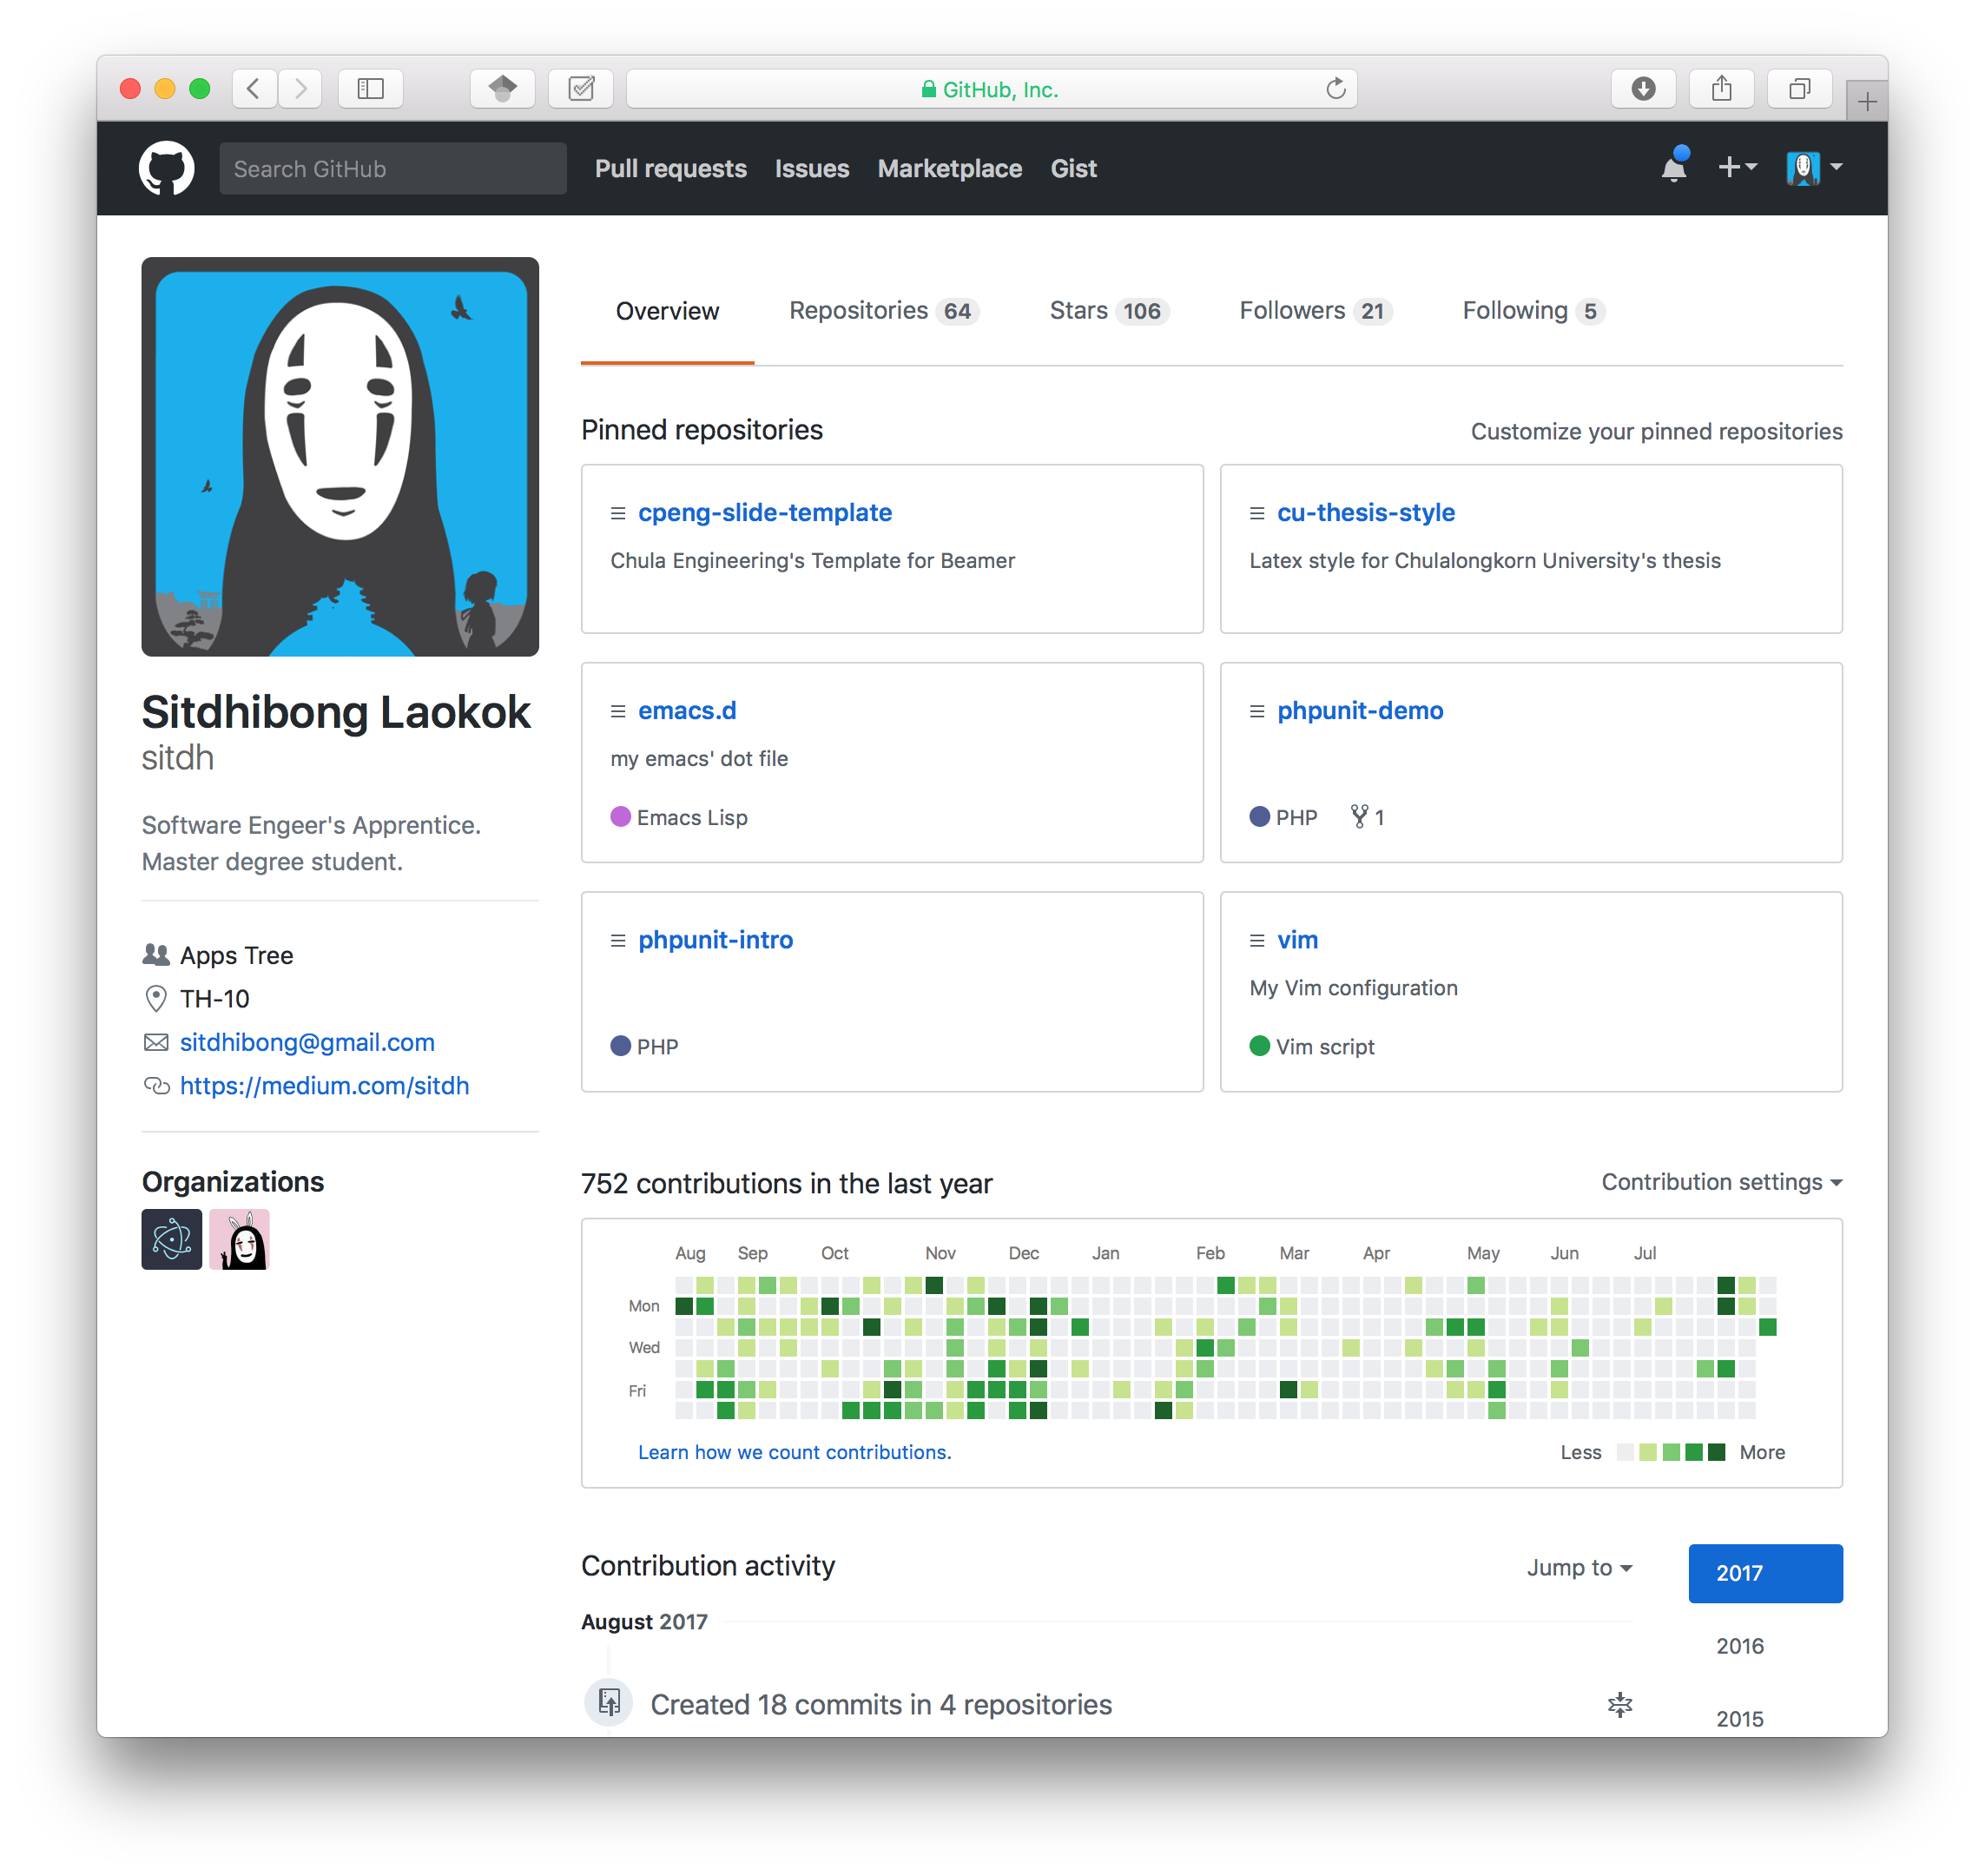
\includegraphics[width=.8\textwidth]{git-profile}
        \caption{https://github.com/sitdh}
        \label{fig:git-profile}
    \end{figure}
\end{frame}

\begin{frame}{Outline}
    \tableofcontents
\end{frame}

\begin{frame}{Hello}
    \begin{figure}
        \center
        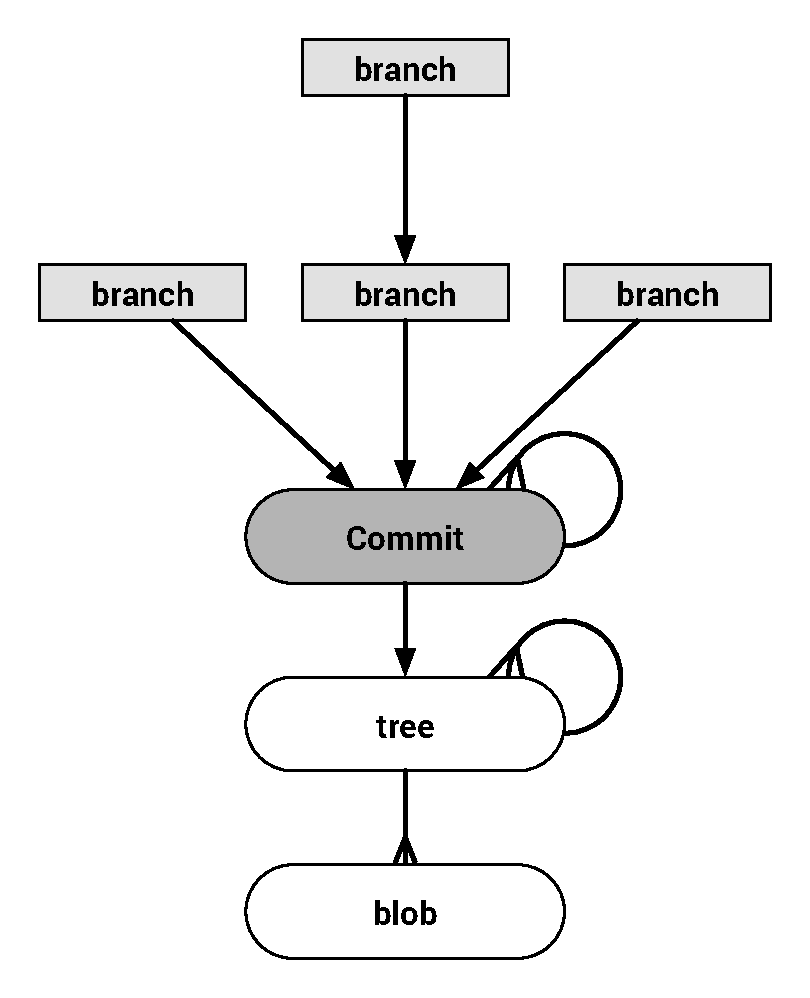
\includegraphics[height=.8\textheight]{git-action}
        \label{fig:git-action}
    \end{figure}
\end{frame}

\section{init}
\begin{frame}{Command flow}
    \begin{figure}
        \center
        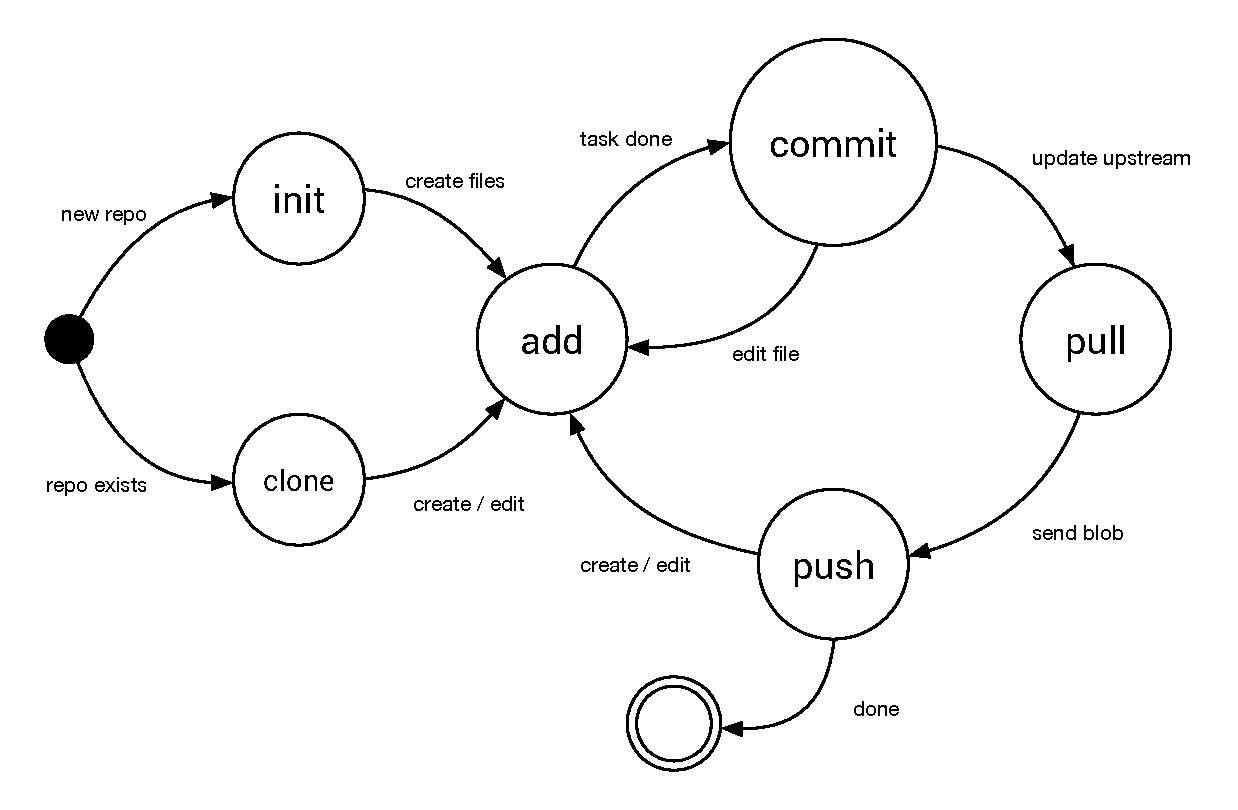
\includegraphics[width=.9\textwidth]{git-command-flow}
        \label{fig:git-action}
    \end{figure}
\end{frame}

\section{clone}

\section{add}

\section{commit}

\section{pull}

\section{push}

\section{Checkup}
\begin{frame}{Checkup}
    \begin{figure}
        \center
        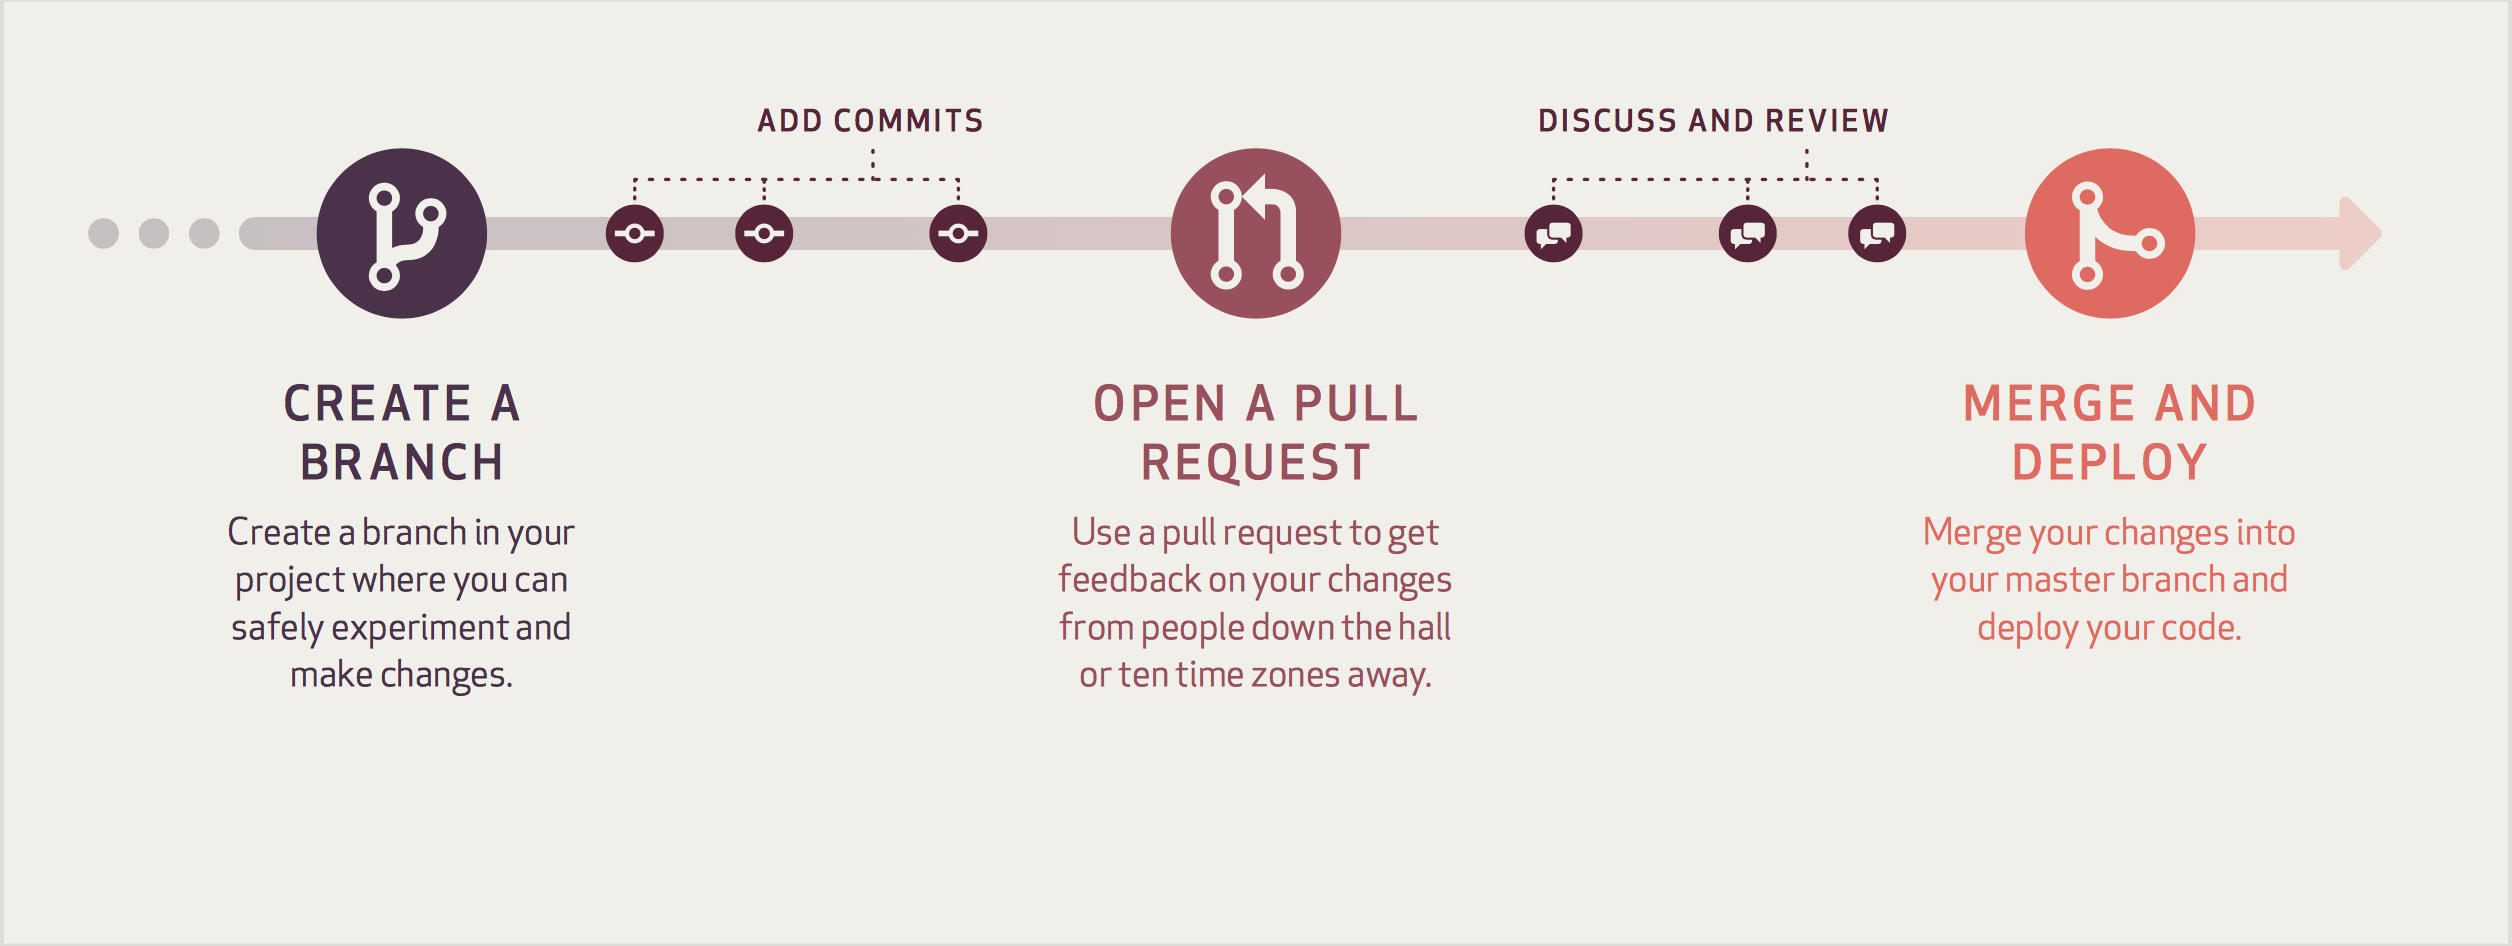
\includegraphics[width=.9\textwidth]{git-workflow}
        \caption{https://guides.github.com/introduction/flow/}
        \label{fig:git-workflow}
    \end{figure}
\end{frame}

\end{document}
